% This file was created by matplotlib2tikz v0.6.18.
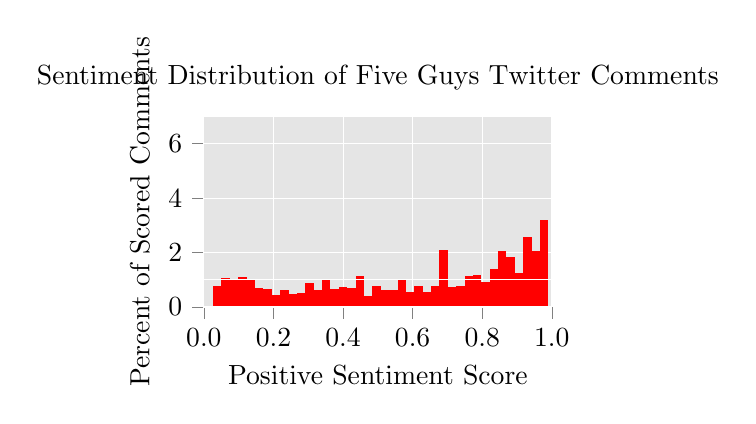
\begin{tikzpicture}

\begin{axis}[
axis background/.style={fill=white!89.80392156862746!black},
axis line style={white},
height=4cm,
tick align=outside,
tick pos=left,
title={Sentiment Distribution of Five Guys Twitter Comments},
width=6cm,
x grid style={white},
xlabel={Positive Sentiment Score},
xmajorgrids,
xmin=0, xmax=1,
xtick={0,0.2,0.4,0.6,0.8,1},
xticklabels={0.0,0.2,0.4,0.6,0.8,1.0},
y grid style={white},
ylabel={Percent of Scored Comments},
ymajorgrids,
ymin=0, ymax=7
]
\draw[fill=red,draw opacity=0] (axis cs:0.0264586992561817,0) rectangle (axis cs:0.0505512282252312,0.778249617285513);
\draw[fill=red,draw opacity=0] (axis cs:0.0505512282252312,0) rectangle (axis cs:0.0746437609195709,1.07009314103638);
\draw[fill=red,draw opacity=0] (axis cs:0.0746437534689903,0) rectangle (axis cs:0.0987362787127495,1.0376662366049);
\draw[fill=red,draw opacity=0] (axis cs:0.0987362861633301,0) rectangle (axis cs:0.12282881885767,1.10252003543988);
\draw[fill=red,draw opacity=0] (axis cs:0.122828811407089,0) rectangle (axis cs:0.146921336650848,1.0376662366049);
\draw[fill=red,draw opacity=0] (axis cs:0.146921336650848,0) rectangle (axis cs:0.171013861894608,0.680968467771963);
\draw[fill=red,draw opacity=0] (axis cs:0.171013861894608,0) rectangle (axis cs:0.195106387138367,0.64854139787806);
\draw[fill=red,draw opacity=0] (axis cs:0.195106387138367,0) rectangle (axis cs:0.219198912382126,0.453978978514642);
\draw[fill=red,draw opacity=0] (axis cs:0.219198912382126,0) rectangle (axis cs:0.243291452527046,0.61611394691936);
\draw[fill=red,draw opacity=0] (axis cs:0.243291467428207,0) rectangle (axis cs:0.267383992671967,0.486406349249546);
\draw[fill=red,draw opacity=0] (axis cs:0.267383962869644,0) rectangle (axis cs:0.291476517915726,0.518832476509503);
\draw[fill=red,draw opacity=0] (axis cs:0.291476488113403,0) rectangle (axis cs:0.315569013357162,0.87553088713538);
\draw[fill=red,draw opacity=0] (axis cs:0.315569043159485,0) rectangle (axis cs:0.339661568403244,0.616114327984157);
\draw[fill=red,draw opacity=0] (axis cs:0.339661538600922,0) rectangle (axis cs:0.363754063844681,1.0376662366049);
\draw[fill=red,draw opacity=0] (axis cs:0.363754093647003,0) rectangle (axis cs:0.387846618890762,0.64854139787806);
\draw[fill=red,draw opacity=0] (axis cs:0.38784658908844,0) rectangle (axis cs:0.411939114332199,0.745822607559768);
\draw[fill=red,draw opacity=0] (axis cs:0.411939144134521,0) rectangle (axis cs:0.436031669378281,0.680968467771963);
\draw[fill=red,draw opacity=0] (axis cs:0.436031639575958,0) rectangle (axis cs:0.460124164819717,1.1349474462866);
\draw[fill=red,draw opacity=0] (axis cs:0.46012419462204,0) rectangle (axis cs:0.484216719865799,0.389124838726836);
\draw[fill=red,draw opacity=0] (axis cs:0.484216690063477,0) rectangle (axis cs:0.508309245109558,0.778249677453671);
\draw[fill=red,draw opacity=0] (axis cs:0.508309245109558,0) rectangle (axis cs:0.53240180015564,0.616113565855034);
\draw[fill=red,draw opacity=0] (axis cs:0.53240180015564,0) rectangle (axis cs:0.556494295597076,0.616115090115164);
\draw[fill=red,draw opacity=0] (axis cs:0.556494295597076,0) rectangle (axis cs:0.580586850643158,1.03766495301901);
\draw[fill=red,draw opacity=0] (axis cs:0.580586910247803,0) rectangle (axis cs:0.60467940568924,0.551260870103042);
\draw[fill=red,draw opacity=0] (axis cs:0.604679346084595,0) rectangle (axis cs:0.628771901130676,0.778248714764254);
\draw[fill=red,draw opacity=0] (axis cs:0.628771901130676,0) rectangle (axis cs:0.652864396572113,0.551260870103042);
\draw[fill=red,draw opacity=0] (axis cs:0.652864396572113,0) rectangle (axis cs:0.676956951618195,0.778248714764254);
\draw[fill=red,draw opacity=0] (axis cs:0.676957011222839,0) rectangle (axis cs:0.701049506664276,2.10776215039398);
\draw[fill=red,draw opacity=0] (axis cs:0.701049447059631,0) rectangle (axis cs:0.725142002105713,0.74582168498241);
\draw[fill=red,draw opacity=0] (axis cs:0.725142002105713,0) rectangle (axis cs:0.749234557151794,0.778248714764254);
\draw[fill=red,draw opacity=0] (axis cs:0.749234557151794,0) rectangle (axis cs:0.773327052593231,1.13494885021214);
\draw[fill=red,draw opacity=0] (axis cs:0.773327052593231,0) rectangle (axis cs:0.797419607639313,1.16737307214638);
\draw[fill=red,draw opacity=0] (axis cs:0.797419667243958,0) rectangle (axis cs:0.821512162685394,0.907959080169716);
\draw[fill=red,draw opacity=0] (axis cs:0.82151210308075,0) rectangle (axis cs:0.845604658126831,1.39436228061929);
\draw[fill=red,draw opacity=0] (axis cs:0.845604658126831,0) rectangle (axis cs:0.869697153568268,2.04290793038186);
\draw[fill=red,draw opacity=0] (axis cs:0.869697153568268,0) rectangle (axis cs:0.893789708614349,1.8483406975651);
\draw[fill=red,draw opacity=0] (axis cs:0.893789768218994,0) rectangle (axis cs:0.917882263660431,1.26465729023639);
\draw[fill=red,draw opacity=0] (axis cs:0.917882204055786,0) rectangle (axis cs:0.941974759101868,2.56173535276567);
\draw[fill=red,draw opacity=0] (axis cs:0.941974759101868,0) rectangle (axis cs:0.966067254543304,2.07533504038792);
\draw[fill=red,draw opacity=0] (axis cs:0.966067254543304,0) rectangle (axis cs:0.990159809589386,3.21027594840255);
\path [draw=white, fill opacity=0] (axis cs:0,0)
--(axis cs:0,7);

\path [draw=white, fill opacity=0] (axis cs:1,0)
--(axis cs:1,7);

\path [draw=white, fill opacity=0] (axis cs:0,0)
--(axis cs:1,0);

\path [draw=white, fill opacity=0] (axis cs:0,1)
--(axis cs:1,1);

\end{axis}

\end{tikzpicture}